\documentclass[12pt]{article}

% custom commands
\newcommand{\paren}[1]{\left( {#1} \right)}
\newcommand{\abs}[1]{\left| {#1} \right|}

% Math and symbol packages
\usepackage{amsmath}
\usepackage{amssymb}
\usepackage{derivative}

% Figure Packages
\usepackage{graphicx}
\usepackage{wrapfig}
\usepackage{epstopdf}
\usepackage{float}
\usepackage{subfigure}
\usepackage{lipsum}
\usepackage{caption}
\usepackage{subcaption}
\usepackage{booktabs}

% Formatting and Random Text Generation
\usepackage{inputenc}
\usepackage[left=2.54cm,right=2.54cm,top=2.54cm,bottom=2.54cm]{geometry}
\usepackage{lipsum}

% Header and indent packages
\usepackage{fancyhdr}
\usepackage{indentfirst}

% Create Title Section
\title{Damped and Forced Oscillators \\ \small (LCR)}
\author{Trevor Swan \\
Department of Physics, Case Western Reserve University \\
Cleveland, OH 44016-7079}
\date{4/15/25}

% Create paragraph formatting
%\setlength{\parindent}{3em}

% Actual Lab content
\begin{document}
\pagestyle{fancy}
\fancyhf{}

% Load the title
\maketitle
\thispagestyle{fancy}
\renewcommand{\headrulewidth}{0pt}

% Set up Footers
\fancyfoot[L]{Trevor Swan}
\fancyfoot[C]{\thepage}
\fancyfoot[R]{Damped and Forced Oscillators}

% Abstract section of Report
\section{Abstract}
\lipsum[1]

% Introduction and Thoery
\section{Introduction and Theory}
\lipsum[1]

% Procedure
\section{Experimental Procedure}
\subsection{Damped Oscillator}
\lipsum[1]

\begin{wrapfigure}{r}{0.5\textwidth}
    \centering
    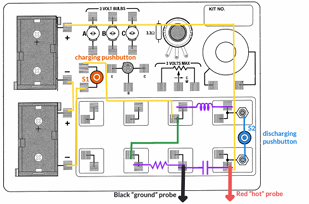
\includegraphics[width=\linewidth]{figures/images/LCR_Apparatus_1.png}
    \caption{Experimental Apparatus of Damped Oscillator section from the LCR Lab Manual \ref{ref:MANUEL}}
    \label{fig:LCR_Apparatus_1}
\end{wrapfigure}

\lipsum[1]

\subsection{Resonant Circuit}
\lipsum[1]

\begin{wrapfigure}{r}{0.5\textwidth}
    \centering
    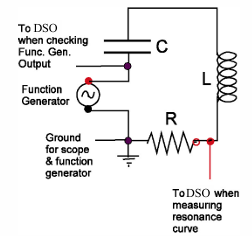
\includegraphics[width=\linewidth]{figures/images/LCR_Apparatus_2.png}
    \caption{Experimental Apparatus of Resonant Circuit section from the LCR Lab Manual \ref{ref:MANUEL}}
    \label{fig:LCR_Apparatus_2}
\end{wrapfigure}

\lipsum[1]

% Results and Analysis
\section{Results and Analysis}
\lipsum[1]

% Conclusion
\section{Conclusion}
\lipsum[1]

\subsection{Acknowledgments}
I would like to thank Pratham Bhashyakarla, CWRU Department of Physics, for his help in obtaining the experimental data, preparing the figures, and checking my calculations.

\subsection{References}
\begin{enumerate}
    \item Driscoll, D., General Physics II: E$\&$M Lab Manual, “Damped and Forced Oscillators,” CWRU Bookstore, 2016.
    \label{ref:MANUEL}
\end{enumerate}

\clearpage
\appendix
\section{Appendix}
\addcontentsline{toc}{section}{Appendix}
\subsection{Damped Oscillator}

\begin{table}[h]
\centering
\begin{tabular}{|c|c|c|c|}
\hline
\textbf{A (V)} & \textbf{L (s)} & $\omega$ \textbf{(1/s)} & \textbf{P (unitless)} \\
\hline
$-7.94 \pm 0.12$  & $0.00078 \pm 2*10^{-5}$  & $2.30*10^4 \pm 22$ & $-0.199 \pm 0.14$ \\
\hline
\end{tabular}
\caption{Trial data generated from Logger Pro, presented in Figure \ref{fig:D1_022C_0R}. This data will be referred to as 'Trial 1's data'.}
\label{tab:damped_trial_1}
\end{table}

\begin{table}[h]
\centering
\begin{tabular}{|c|c|c|c|}
\hline
\textbf{A (V)} & \textbf{L (s)} & $\omega$ \textbf{(1/s)} & \textbf{P (unitless)} \\
\hline
$-6.17 \pm 0.03$  & $0.00086 \pm 5*10^{-6}$  & $4912 \pm 5$ & $0.275 \pm 0.004$ \\
\hline
\end{tabular}
\caption{Trial data generated from Logger Pro, presented in Figure \ref{fig:D2_47C_0R}. This data will be referred to as 'Trial 2's data'.}
\label{tab:damped_trial_2}
\end{table}

\begin{table}[h]
\centering
\begin{tabular}{|c|c|c|c|}
\hline
\textbf{A (V)} & \textbf{L (s)} & $\omega$ \textbf{(1/s)} & \textbf{P (unitless)} \\
\hline
$908.0 \pm 1.3$  & $0.00058 \pm 5*10^{-7}$  & $4724 \pm 1.3$ & $-1.425 \pm 0.005$ \\
\hline
\end{tabular}
\caption{Trial data generated from Logger Pro, presented in Figure \ref{fig:D3_47C_100R}. This data will be referred to as 'Trial 1's data'.}
\label{tab:damped_trial_3}
\end{table}

\begin{table}[h]
\centering
\begin{tabular}{|c|c|c|c|}
\hline
\textbf{A (V)} & \textbf{L (s)} & $\omega$ \textbf{(1/s)} & \textbf{P (unitless)} \\
\hline
$7.53 \pm 0.07$  & $0.00024 \pm 2*10^{-6}$  & $-2829 \pm 3$ & $-0.337 \pm 0.002$ \\
\hline
\end{tabular}
\caption{Trial data generated from Logger Pro, presented in Figure \ref{fig:D4_47C_500R}. This data will be referred to as 'Trial 1's data'.}
\label{tab:damped_trial_4}
\end{table}

\begin{table}[h]
\centering
\begin{tabular}{|c|c|c|c|}
\hline
\textbf{A (V)} & \textbf{L (s)} & $\omega$ \textbf{(1/s)} & \textbf{P (unitless)} \\
\hline
$-22.5 \pm 3.0$  & $0.00011 \pm 1*10^{-6}$  & $-0.0002*10^4 \pm 3$ & $0.12 \pm 0.02$ \\
\hline
\end{tabular}
\caption{Trial data generated from Logger Pro, presented in Figure \ref{fig:D5_47C_1000R}. This data will be referred to as 'Trial 1's data'.}
\label{tab:damped_trial_5}
\end{table}

\begin{table}[h]
\centering
\begin{tabular}{|c|c|c|c|}
\hline
\textbf{A (V)} & \textbf{L (s)} & $\omega$ \textbf{(1/s)} & \textbf{P (unitless)} \\
\hline
$-751.9 \pm 9.6$  & $0.0007 \pm 0.0006$  & $-3.55*10^{-7} \pm 10$ & $0.0107 \pm 0.0004$ \\
\hline
\end{tabular}
\caption{Trial data generated from Logger Pro, presented in Figure \ref{fig:D6_47C_2000R}. This data will be referred to as 'Trial 1's data'.}
\label{tab:damped_trial_6}
\end{table}

\begin{figure} [h]
    \begin{subfigure}
        \centering
        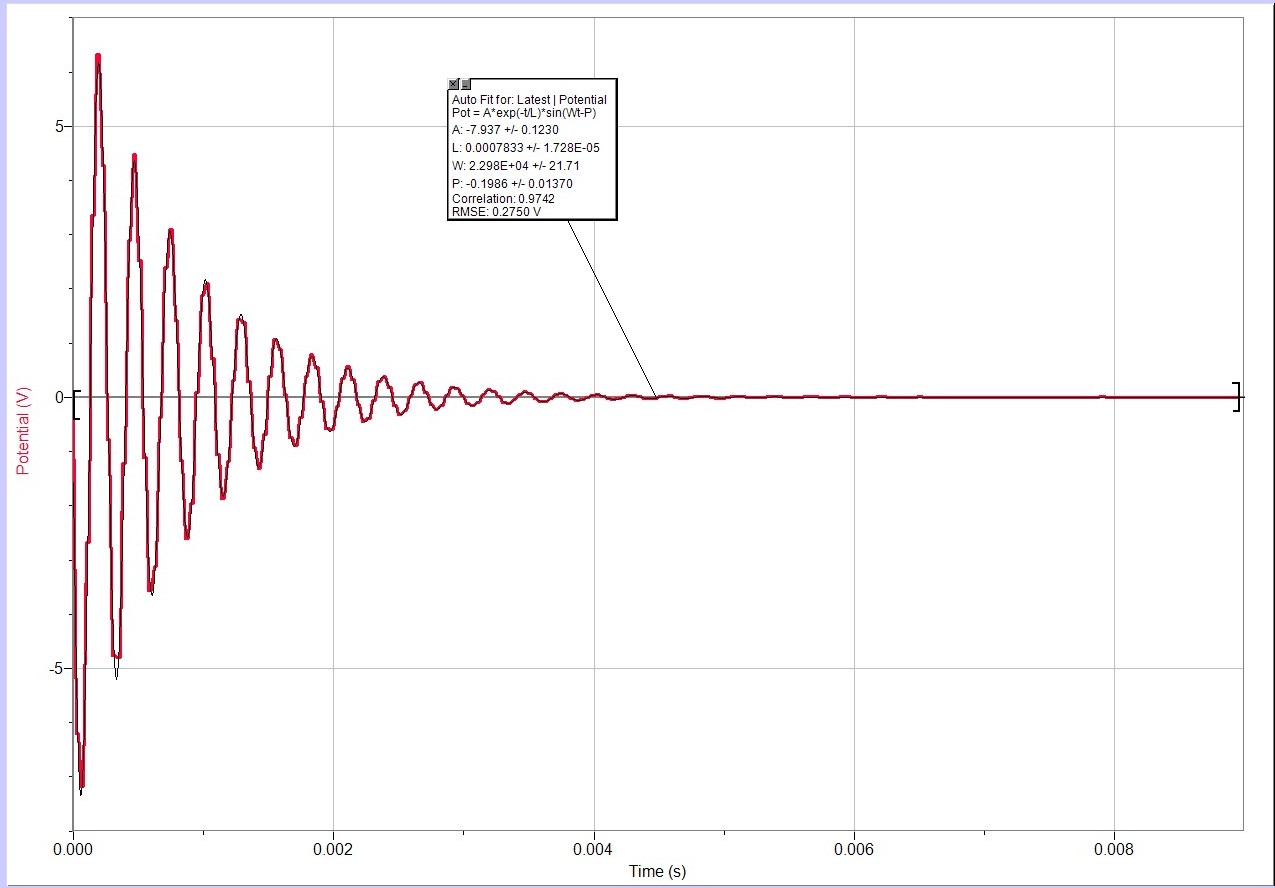
\includegraphics[width=0.7\textwidth]{figures/images/LCR_D1_Logger-Plot.jpg}
        \caption{Damped Oscillator plot using Logger Pro of the charge stored in a capacitor inside a circuit with a 0.022 $\mu$ F capacitor and no resistor. The capacitor was measured to have a capacitance of $0.022\pm0.001\mu$ F. There is also an $86.6\pm0.1$mH inductor in the circuit.}
        \label{fig:D1_022C_0R}
    \end{subfigure}
\end{figure}

\begin{figure} [h]
    \begin{subfigure}
        \centering
        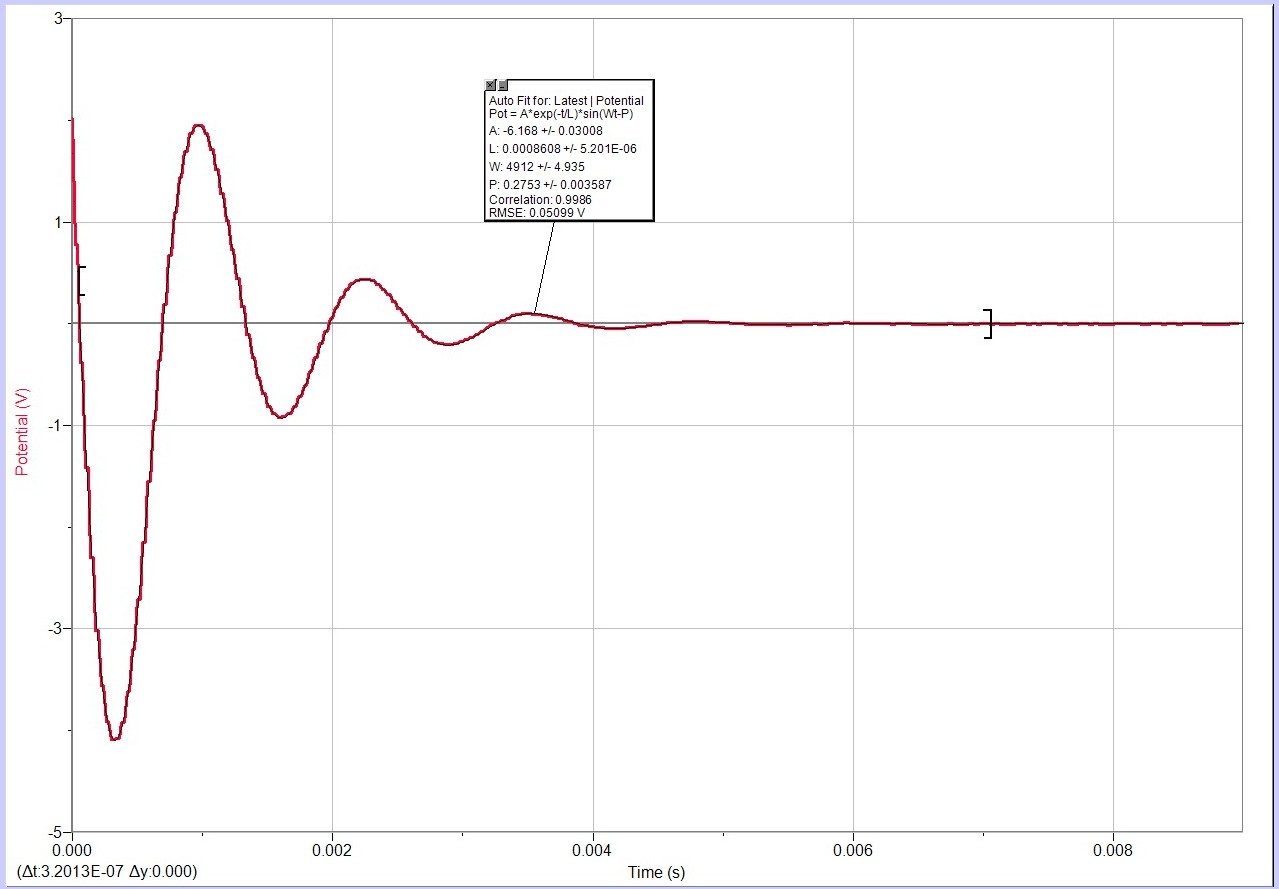
\includegraphics[width=0.7\textwidth]{figures/images/LCR_D2_Logger-Plot.jpg}
        \caption{Damped Oscillator plot using Logger Pro of the charge stored in a capacitor inside a circuit with a 0.47 $\mu$ F capacitor and no resistor. The capacitor was measured to have a capacitance of $0.47\pm0.01\mu$ F. There is also an $86.6\pm0.1$mH inductor in the circuit.}
        \label{fig:D2_47C_0R}
    \end{subfigure}
\end{figure}

\begin{figure} [h]
    \begin{subfigure}
        \centering
        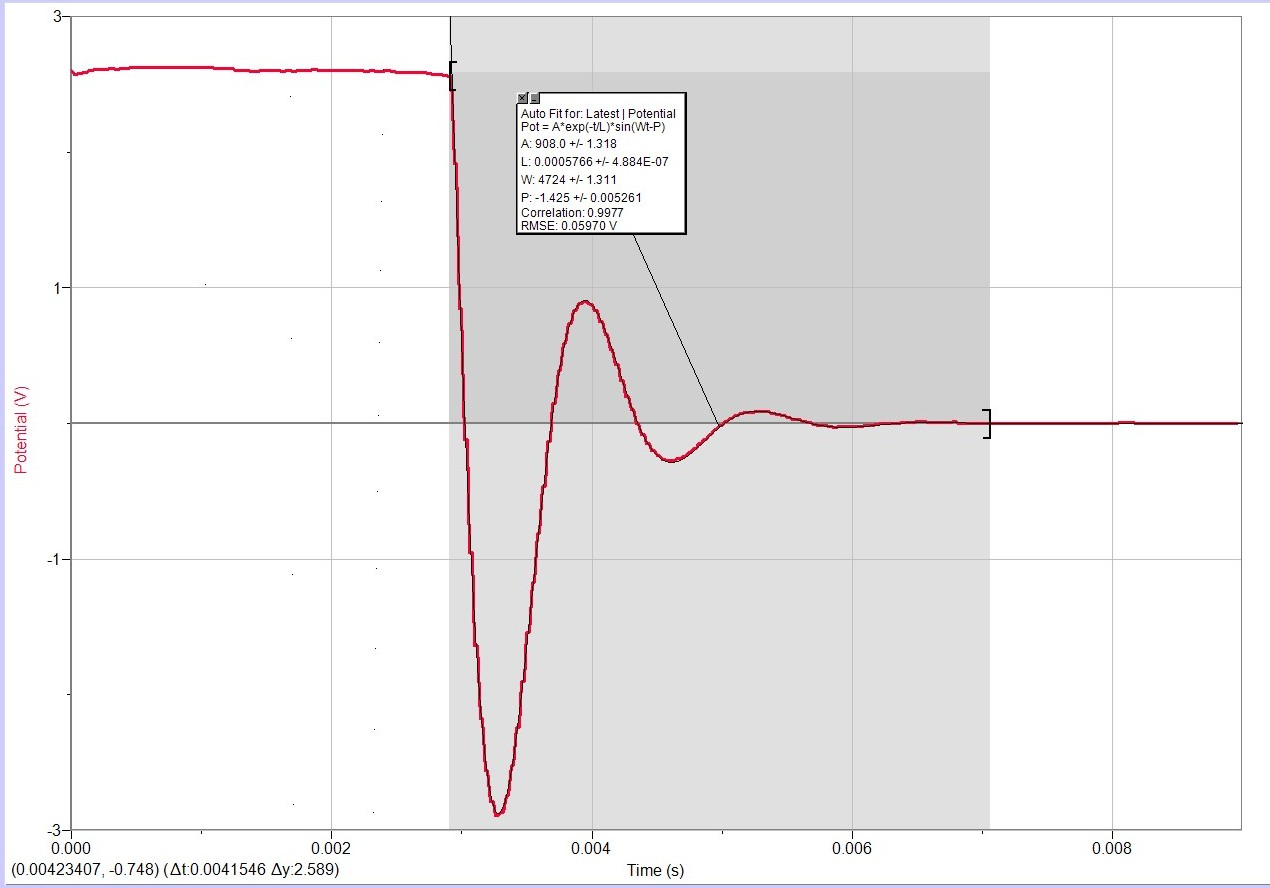
\includegraphics[width=0.7\textwidth]{figures/images/LCR_D3_Logger-Plot.jpg}
        \caption{Damped Oscillator plot using Logger Pro of the charge stored in a capacitor inside a circuit with a 0.47 $\mu$ F capacitor and a 100$\Omega$ resistor. The capacitor was measured to have a capacitance of $0.47\pm0.01\mu$ F, and the resistor was measured to have a resistance of $99.1\pm0.1\Omega$. There is also an $86.6\pm0.1$mH inductor in the circuit.}
        \label{fig:D3_47C_100R}
    \end{subfigure}
\end{figure}

\begin{figure} [h]
    \begin{subfigure}
        \centering
        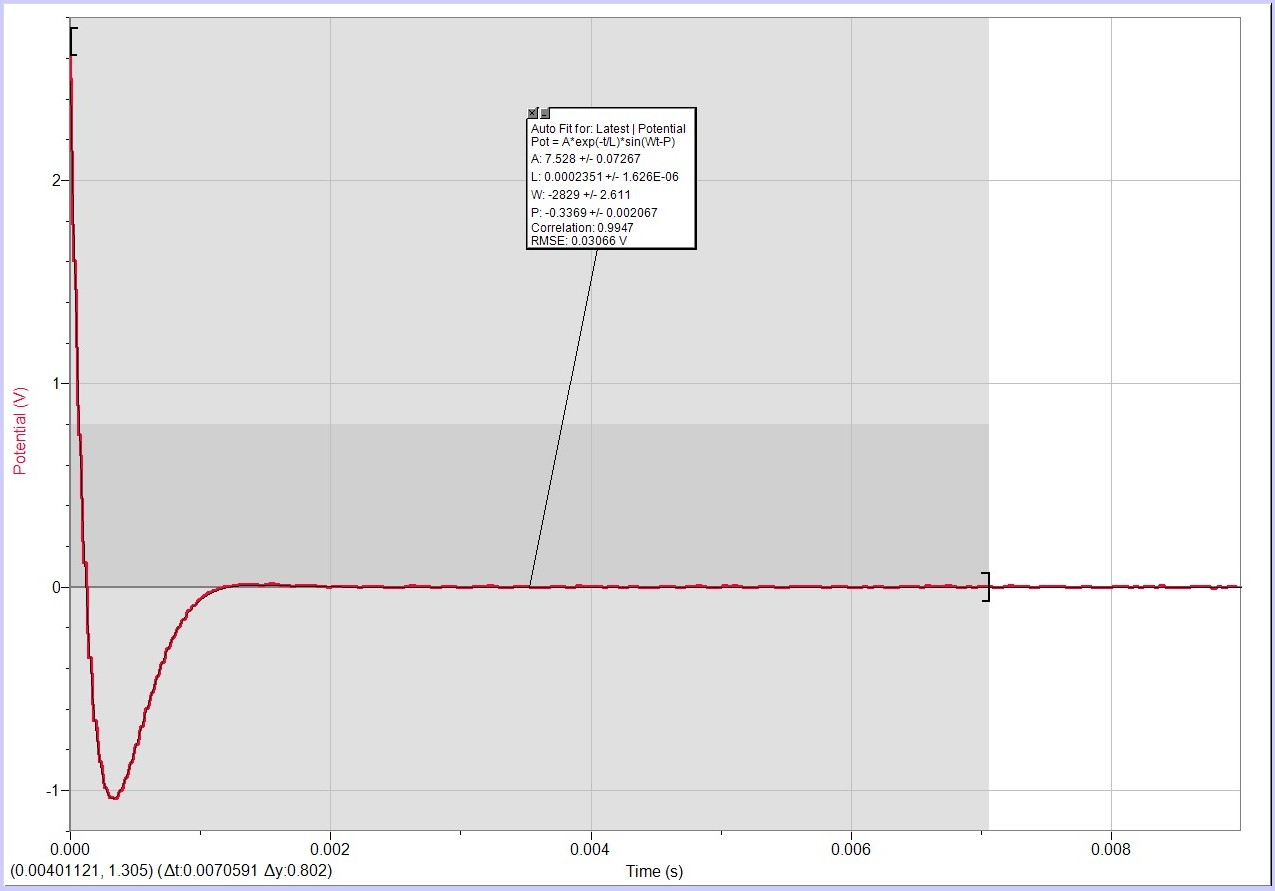
\includegraphics[width=0.7\textwidth]{figures/images/LCR_D4_Logger-Plot.jpg}
        \caption{Damped Oscillator plot using Logger Pro of the charge stored in a capacitor inside a circuit with a 0.47 $\mu$ F capacitor and a 500$\Omega$ resistor. The capacitor was measured to have a capacitance of $0.47\pm0.01\mu$ F, and the resistor was measured to have a resistance of $492.5\pm0.1\Omega$. This resistor was created by combining two resistors in parallel, measuring $0.99\pm0.01\text{k}\Omega$ and $0.98\pm0.01\text{k}\Omega$, respectively. There is also an $86.6\pm0.1$mH inductor in the circuit.}
        \label{fig:D4_47C_500R}
    \end{subfigure}
\end{figure}

\begin{figure} [h]
    \begin{subfigure}
        \centering
        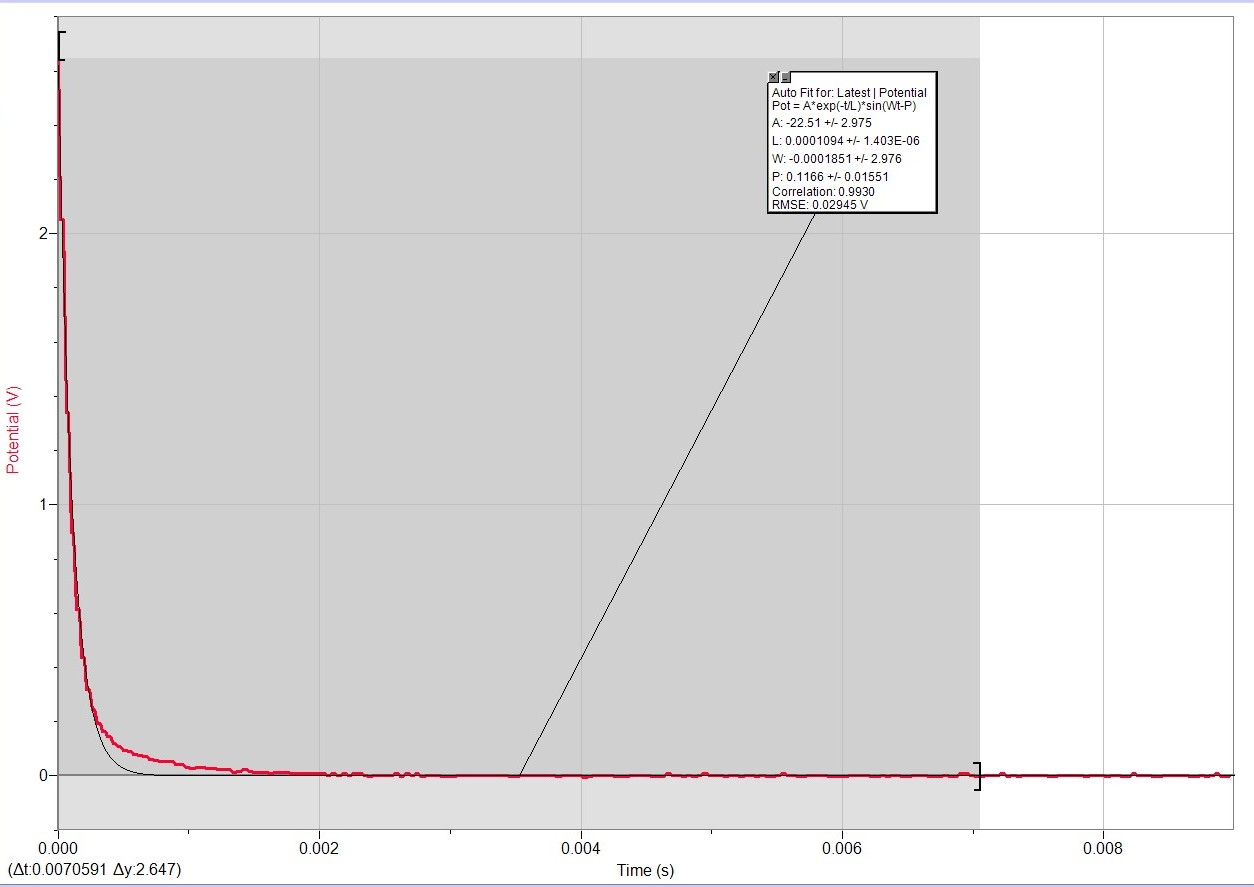
\includegraphics[width=0.7\textwidth]{figures/images/LCR_D5_Logger-Plot.jpg}
        \caption{Damped Oscillator plot using Logger Pro of the charge stored in a capacitor inside a circuit with a 0.47 $\mu$ F capacitor and a 1 k$\Omega$ resistor. The capacitor was measured to have a capacitance of $0.47\pm0.01\mu$ F, and the resistor was measured to have a resistance of $0.99\pm0.01\text{k}\Omega$. There is also an $86.6\pm0.1$mH inductor in the circuit.}
        \label{fig:D5_47C_1000R}
    \end{subfigure}
\end{figure}

\begin{figure} [h]
    \begin{subfigure}
        \centering
        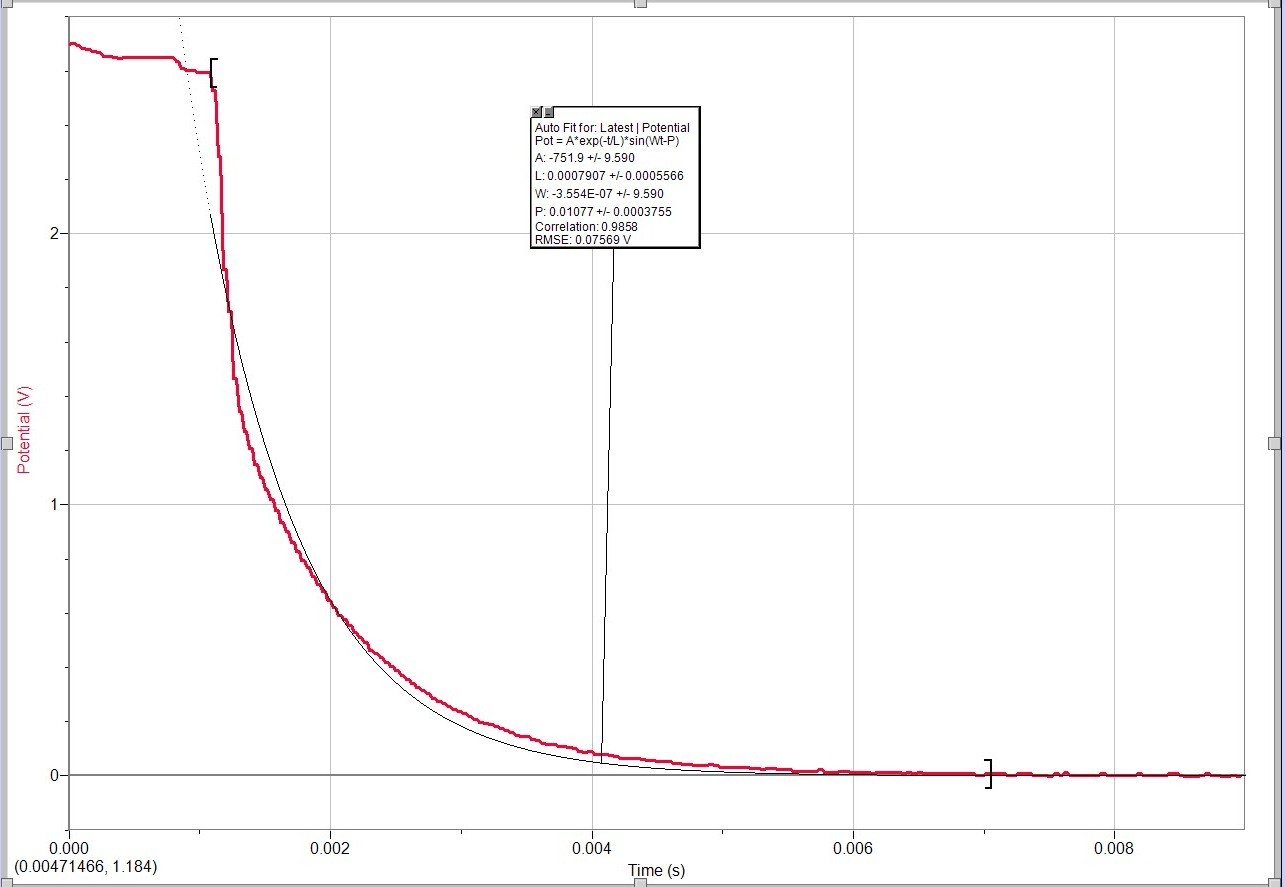
\includegraphics[width=0.7\textwidth]{figures/images/LCR_D6_Logger-Plot.jpg}
        \caption{Damped Oscillator plot using Logger Pro of the charge stored in a capacitor inside a circuit with a 0.47 $\mu$ F capacitor and a 1 k$\Omega$ resistor. The capacitor was measured to have a capacitance of $0.47\pm0.01\mu$ F, and the resistor was measured to have a resistance of $1.97\pm0.02\text{k}\Omega$. This resistor was created by combining two resistors in series, measuring $0.99\pm0.01\text{k}\Omega$ and $0.98\pm0.01\text{k}\Omega$, respectively. There is also an $86.6\pm0.1$mH inductor in the circuit.}
        \label{fig:D6_47C_2000R}
    \end{subfigure}
\end{figure}

\clearpage
\subsection{Resonant Circuit}

\begin{table}[h]
\centering
\begin{tabular}{|c|c|c|}
\hline
\textbf{Frequency (Hz)} & \textbf{Vpp (V)} & \textbf{Gain} \\
\hline
$2.25 \pm 0.01$  & $1.14 \pm 0.02$  & $0.07125 \pm 0.00125$ \\
$3.55 \pm 0.01$  & $2.02 \pm 0.02$  & $0.12625 \pm 0.00125$ \\
$4.85 \pm 0.01$  & $3.34 \pm 0.02$  & $0.20875 \pm 0.00125$ \\
$6.15 \pm 0.01$  & $5.10 \pm 0.02$  & $0.31875 \pm 0.00125$ \\
$7.45 \pm 0.01$  & $10.40 \pm 0.02$ & $0.65000 \pm 0.00125$ \\
$8.00 \pm 0.01$  & $10.96 \pm 0.02$ & $0.68500 \pm 0.00125$ \\
$8.75 \pm 0.01$  & $9.92 \pm 0.02$  & $0.62000 \pm 0.00125$ \\
$10.05 \pm 0.01$ & $6.88 \pm 0.02$  & $0.43000 \pm 0.00125$ \\
$11.35 \pm 0.01$ & $4.96 \pm 0.02$  & $0.31000 \pm 0.00125$ \\
$12.65 \pm 0.01$ & $3.92 \pm 0.02$  & $0.24500 \pm 0.00125$ \\
$13.95 \pm 0.01$ & $3.20 \pm 0.02$  & $0.20000 \pm 0.00125$ \\
$15.25 \pm 0.01$ & $2.72 \pm 0.02$  & $0.17000 \pm 0.00125$ \\
$16.55 \pm 0.01$ & $2.40 \pm 0.02$  & $0.15000 \pm 0.00125$ \\
$17.85 \pm 0.01$ & $2.16 \pm 0.02$  & $0.13500 \pm 0.00125$ \\
$19.15 \pm 0.01$ & $1.92 \pm 0.02$  & $0.12000 \pm 0.00125$ \\
$20.45 \pm 0.01$ & $1.76 \pm 0.02$  & $0.11000 \pm 0.00125$ \\
$21.75 \pm 0.01$ & $1.68 \pm 0.02$  & $0.10500 \pm 0.00125$ \\
$23.05 \pm 0.01$ & $1.52 \pm 0.02$  & $0.09500 \pm 0.00125$ \\
$24.35 \pm 0.01$ & $1.39 \pm 0.02$  & $0.08688 \pm 0.00125$ \\
$25.65 \pm 0.01$ & $1.31 \pm 0.02$  & $0.08188 \pm 0.00125$ \\
$26.95 \pm 0.01$ & $1.23 \pm 0.02$  & $0.07688 \pm 0.00125$ \\
$28.25 \pm 0.01$ & $1.18 \pm 0.02$  & $0.07375 \pm 0.00125$ \\
$29.00 \pm 0.01$ & $1.12 \pm 0.02$  & $0.07000 \pm 0.00125$ \\
\hline
\end{tabular}
\caption{Frequency vs. Vpp and Gain with uncertainties. Gain and its uncertainty is calculated by dividing the corresponding Vpp values by 16, the input voltage from the function generator. }
\label{tab:gain_freq}
\end{table}

\begin{figure} [h]
    \begin{subfigure}
        \centering
        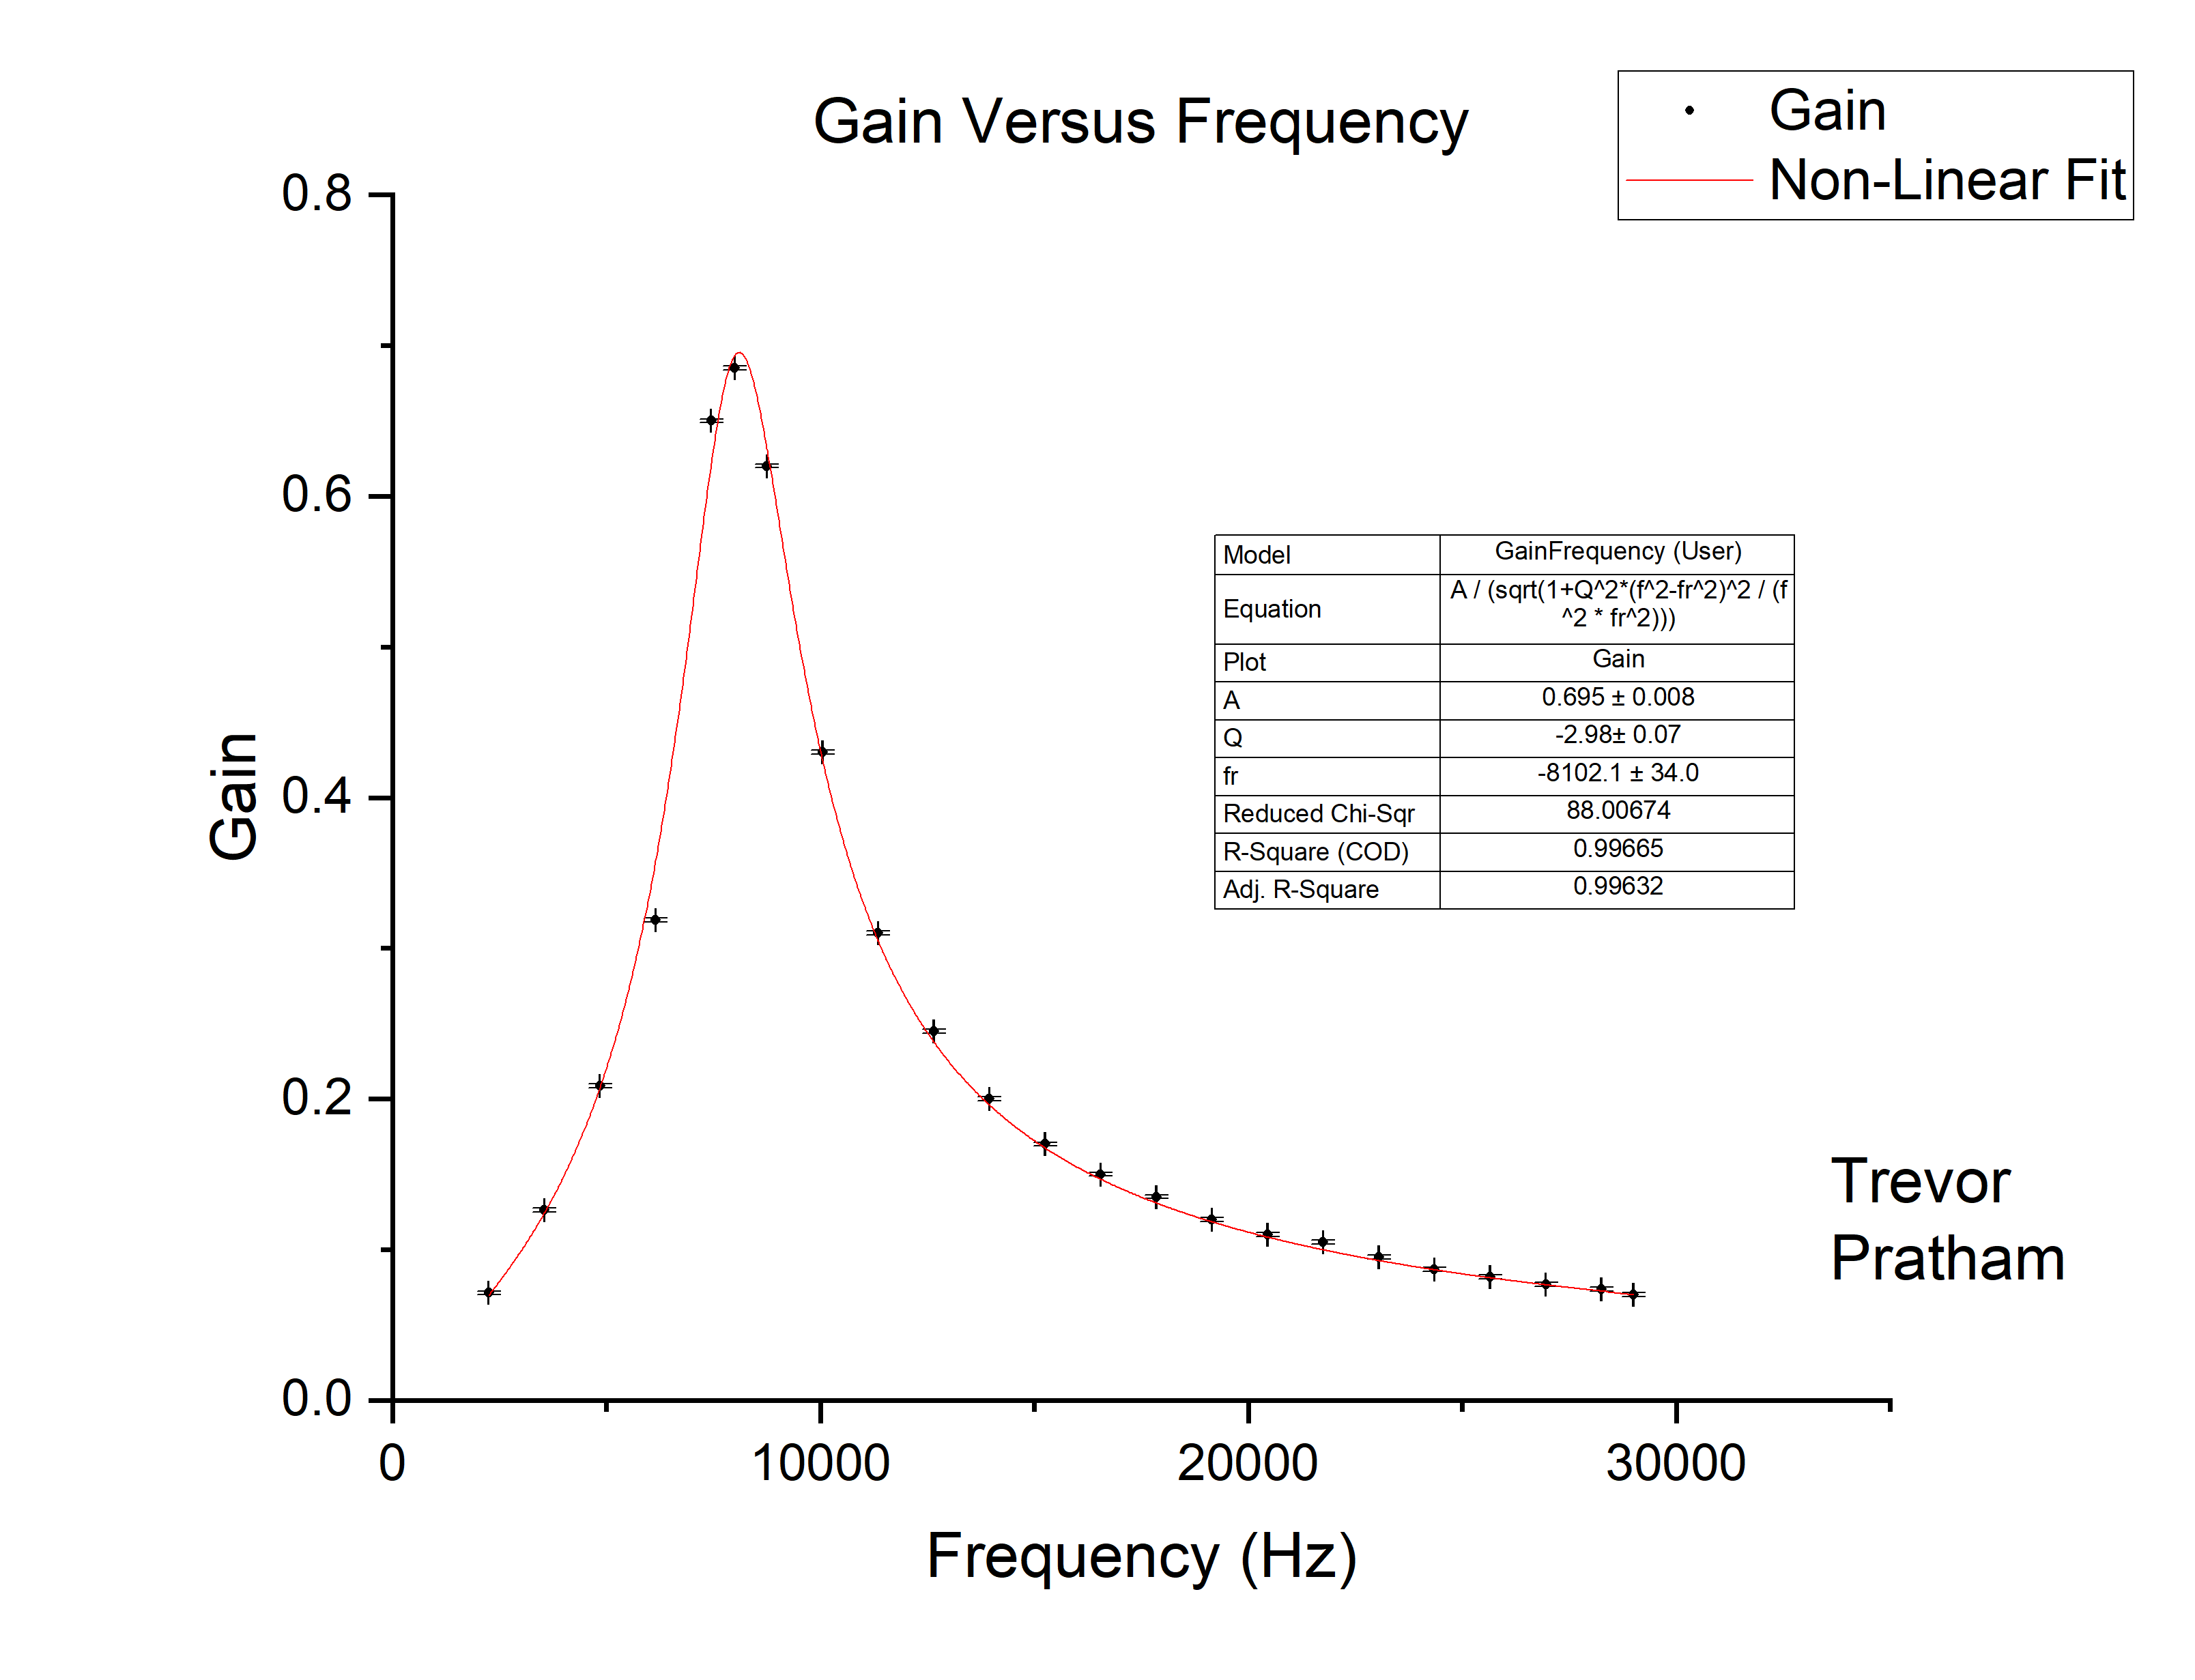
\includegraphics[width=0.7\textwidth]{figures/images/LCR_Gain-Frequency.png}
        \caption{Plot of Gain vs. Frequency from the above table (Table \ref{tab:gain_freq}). Non-linear fit was made using Origin, and the fitting equation along with its parameters are explained in the Theory section of this paper.}
        \label{fig:origin}
    \end{subfigure}
\end{figure}
\clearpage

\section{General Data}

\begin{table}[h]
\centering
\begin{tabular}{|c|c|}
\hline
\textbf{Label} & \textbf{Resistance Value (R)} \\
\hline
$R_1$  & $99.1 \pm 0.1\Omega$ \\
$R_2$  & $990 \pm 10\Omega$ \\
$R_3$  & $980 \pm 10\Omega$ \\
$R_{ind}$  & $188.8 \pm 0.1\Omega$ \\
\hline
\end{tabular}
\caption{Resistance values and their labels used in the appendix.}
\label{tab:resistance_values}
\end{table}

\begin{table}[h]
\centering
\begin{tabular}{|c|c|}
\hline
\textbf{Label} & \textbf{Measured Value (Standard Units)} \\
\hline
$L$  & $0.0866 \pm 0.0001H$ \\
$C_1$  & $2.2*10^{-8} \pm 1*10^{-9}F$ \\
$C_2$  & $4.8*10^{-7} \pm 1*10^{-8}F$ \\
$C_3$  & $4.5*10^{-9} \pm 1*10^{-10}F$ \\
\hline
\end{tabular}
\caption{The inductance (L) is different from the tabulated L values in tables from the previous section. It was calculated by dividing the measured value (in $mH$) by 1000 to get a value in $H$. The capacitance values were determined by dividing the measured values by $10^6$ to get values in terms of $F$. These unit conversions are simple and easy to verbally understand, so they are omitted in this paper. These conversions were made to allow time to be represented in seconds.}
\label{tab:other_measured_values}
\end{table}

\section{Other Calculations}
\subsection{General Resistance Calculations and Error}
\subsubsection{100 Ohm Resistor} \label{subsub:100R}
\begin{align}
R_{eq}=&R_1 + R_{ind}=99.1+188.8=287.9\Omega \nonumber \\
\delta_{R_{eq}}=&\sqrt{\delta_{R_{{eq}_{R_1}}}^2+\delta_{R_{{eq}_{R_{ind}}}}^2} \nonumber \\
=&\sqrt{0.1^2+0.1^2}=0.1 \nonumber \\
R_{eq}=&287.9\pm0.1\Omega \label{eq:100R_w_Inductor}
\end{align}

\subsubsection{500 Ohm Resistor} \label{subsub:500R}
\begin{align}
R_{eq}=&\paren{\frac{1}{R_2}+\frac{1}{R_3}}^{-1} + R_{ind}=\paren{\frac{1}{990}+\frac{1}{980}}^{-1}+188.8=681.3\Omega \nonumber \\
\delta_{R_{eq}}=&\sqrt{\delta_{R_{{eq}_{R_2}}}^2\delta_{R_{{eq}_{R_3}}}^2+\delta_{R_{{eq}_{R_{ind}}}}^2} \nonumber \\
=&\sqrt{0.1^2+0.1^2}=0.1 \nonumber \\
\delta_{R_{{eq}_{R_2}}}=&\frac{\partial}{\partial R_1}\paren{\paren{\frac{1}{R_2}+\frac{1}{R_3}}^{-1} + R_{ind}}*\delta_{R_2} = \frac{R_3^2}{\paren{R_2+R_3}^2} * \delta_{R_2} \nonumber \\
=& \frac{980}{(990+980)^2}*10=2.475 \nonumber \\
\delta_{R_{{eq}_{R_3}}}=&\frac{\partial}{\partial R_2}\paren{\paren{\frac{1}{R_2}+\frac{1}{R_3}}^{-1} + R_{ind}}*\delta_{R_3} = \frac{R_2^2}{\paren{R_2+R_3}^2} * \delta_{R_3} \nonumber \\
=& \frac{990}{(990+980)^2}*10=2.525\nonumber \\
\delta_{R_{{eq}_{R_ind}}}=&\frac{\partial}{\partial R_{ind}}\paren{\paren{\frac{1}{R_2}+\frac{1}{R_3}}^{-1} + R_{ind}}*\delta_{R_{ind}} = \delta_{R_{ind}} = 0.1 \nonumber \\
\delta_{R_{eq}}=&\sqrt{2.475^2+2.525^2+0.1^2}=3.5 \nonumber \\
R_{eq}=&681.3\pm3.5\Omega \label{eq:500R_w_Inductor}
\end{align}

\subsubsection{1000 Ohm Resistor} \label{subsub:1000R_nofunc}
\begin{align}
R_{eq}=&R_2 + R_{ind}=990+188.8=1178.8\Omega \nonumber \\
\delta_{R_{eq}}=&\sqrt{\delta_{R_{{eq}_{R_2}}}^2+\delta_{R_{{eq}_{R_{ind}}}}^2} \nonumber \\
=&\sqrt{10^2+0.1^2}=10 \nonumber \\
R_{eq}=&1178.8\pm10.0\Omega \label{eq:1000R_w_Inductor}
\end{align}

\subsubsection{2000 Ohm Resistor} \label{subsub:2000R}
\begin{align}
R_{eq}=&R_2 + R_3 + R_{ind}=990++980+188.8=2158.8\Omega \nonumber \\
\delta_{R_{eq}}=&\sqrt{\delta_{R_{{eq}_{R_2}}}^2+\delta_{R_{{eq}_{R_3}}}^2+\delta_{R_{{eq}_{R_{ind}}}}^2} \nonumber \\
=&\sqrt{10^2+10^2+0.1^2}=14.1 \nonumber \\
R_{eq}=&2158.8\pm14.1\Omega \label{eq:2000R_w_Inductor}
\end{align}

\subsubsection{1000 Ohm Resistor with Function Generator} \label{subsub:1000R_func}
\begin{align}
R_{eq}=&R_{1000\Omega with Inductor} + R_{Function Generator}=1178.8+50=1228.8\Omega \nonumber \\
\delta_{R_{eq}}=&\sqrt{\delta_{R_{{eq}_{R_{1000\Omega with Inductor}}}}^2+\delta_{R_{{eq}_{R_{Function Generator}}}}^2} \nonumber \\
=&\sqrt{10^2+0^2}=10 \nonumber \\
R_{eq}=&1228.8\pm10.0\Omega \label{eq:1000R_w_Inductor_and_Generator}
\end{align}
The resistance of the function generator is given on the machine to be $50\Omega$. As a result, it is not included with error in the calculation above.

\clearpage
\subsection{Damped Oscillator}
\subsubsection{Generally Useful Expressions}
The following derivation shows the equation and error for $\omega$, the frequency. Derivatives in this section will be taken assuming $L, C, R>0$, which is guaranteed to be true as these are physical properties that are positive by convention.
\begin{align}
	\omega'=&\sqrt{\frac{1}{LC}-\paren{\frac{R}{2L}}^2} \label{eq:omega_prime} \\
	\delta_{\omega'}=&\sqrt{\delta_{\omega'_{L}}^2+\delta_{\omega'_{C}}^2+\delta_{\omega'_{R}}^2}  \label{eq:omega_prime_error} \\
	\delta_{\omega'_{L}}=& \frac{\partial}{\partial L}\paren{\sqrt{\frac{1}{LC}-\paren{\frac{R}{2L}}^2}}*\delta_L=\frac{CR^2-2L}{2L^2\sqrt{C(4L-CR^2)}}*\delta_L \nonumber \\
	\delta_{\omega'_{C}}=& \frac{\partial}{\partial C}\paren{\sqrt{\frac{1}{LC}-\paren{\frac{R}{2L}}^2}}*\delta_C=\frac{1}{C^{3/2}\sqrt{4L-CR^2}}*\delta_C \nonumber \\
	\delta_{\omega'_{R}}=& \frac{\partial}{\partial R}\paren{\sqrt{\frac{1}{LC}-\paren{\frac{R}{2L}}^2}}*\delta_R=\frac{\sqrt{C}R}{2L\sqrt{4L-CR^2}}*\delta_R \nonumber \\
	\delta_{\omega'}=&\sqrt{\paren{\frac{CR^2-2L}{2L^2\sqrt{C(4L-CR^2)}}*\delta_L}^2+\paren{\frac{1}{C^{3/2}\sqrt{4L-CR^2}}*\delta_C}^2+\paren{\frac{\sqrt{C}R}{2L\sqrt{4L-CR^2}}*\delta_R}^2} \label{eq:omega_prime_error_fullexpr}
\end{align}

The following derivation shows the equation and error for $\tau$, the time constant. This is the constant solved for in Logger Pro, given by $L$.
\begin{align}
	\tau=&\frac{2L}{R} \label{eq:tau} \\
	\delta_{\tau}=\sqrt{\delta_{\tau_L}^2+\delta_{\tau_R}^2} \label{eq:tau_error} \\
	\delta_{\tau_L}=&\frac{\partial}{\partial L}\paren{\frac{2L}{R}}*\delta_L = \frac{2}{R}*\delta_L \nonumber \\
	\delta_{\tau_R}=&\frac{\partial}{\partial R}\paren{\frac{2L}{R}}*\delta_R = \frac{2L}{R^2}*\delta_R \nonumber \\
	\delta_{\tau}=& \sqrt{\paren{\frac{2}{R}*\delta_L}^2+\paren{\frac{2L}{R^2}*\delta_R}^2} \label{eq:tau_error_fullexpr}
\end{align}

The following derivation shows the equation and error for $\xi$, the damping coefficient.
\begin{align}
	\xi=&\frac{R}{2}\sqrt{\frac{C}{L}} \label{eq:xi}\\
	\delta_{\xi}=&\sqrt{\delta_{\xi_{L}}^2+\delta_{\xi_{C}}^2+\delta_{\xi_{R}}^2} \label{eq:xi_error} \\
	\delta_{\xi_{L}}=&\frac{\partial}{\partial L}\paren{\frac{R}{2}\sqrt{\frac{C}{L}}}*\delta_L = \frac{R}{4}\sqrt{\frac{C}{L^3}}*\delta_L \nonumber \\
	\delta_{\xi_{C}}=&\frac{\partial}{\partial C}\paren{\frac{R}{2}\sqrt{\frac{C}{L}}}*\delta_C = \frac{R}{4\sqrt{CL}}*\delta_C \nonumber \\
	\delta_{\xi_{R}}=&\frac{\partial}{\partial R}\paren{\frac{R}{2}\sqrt{\frac{C}{L}}}*\delta_R = \frac{1}{2}\sqrt{\frac{C}{L}}*\delta_R \nonumber \\
	\delta_{\xi}=&\sqrt{\paren{\frac{R}{4}\sqrt{\frac{C}{L^3}}*\delta_L}^2+\paren{\frac{R}{4\sqrt{CL}}*\delta_C}^2+\paren{\frac{1}{2}\sqrt{\frac{C}{L}}*\delta_R}^2} \label{ep:xi_error_fullexpr}
\end{align}

\subsubsection{Setup/Trial 1}
Here, we will use values $L=0.0866H$ and $\delta_L=0.0001H$ (Table \ref{tab:other_measured_values}), $C_1$ from Table \ref{tab:other_measured_values}, and $R_{ind}$ from \ref{tab:other_measured_values}. Plugging these values into equations \ref{eq:omega_prime}, \ref{eq:omega_prime_error_fullexpr}, \ref{eq:tau}, \ref{eq:tau_error_fullexpr}, \ref{eq:xi}, and \ref{ep:xi_error_fullexpr} yields:
\begin{align}
	\omega'=22884.3\pm521.4\frac{1}{s} \label{num:omega_prime_trial_one} \\
	\tau=0.000917\pm1.2*10^{-6} s \label{num:tau_trial_one} \\
	\xi=0.048\pm0.001 \label{num:xi_trial_one}
\end{align}

\subsubsection{Setup/Trial 2}
Here, we will use values $L=0.0866H$ and $\delta_L=0.0001H$ (Table \ref{tab:other_measured_values}), $C_2$ from Table \ref{tab:other_measured_values}, and $R_{ind}$ from \ref{tab:other_measured_values}. Plugging these values into equations \ref{eq:omega_prime}, \ref{eq:omega_prime_error_fullexpr}, \ref{eq:tau}, \ref{eq:tau_error_fullexpr}, \ref{eq:xi}, and \ref{ep:xi_error_fullexpr} yields:
\begin{align}
	\omega'=4782.1\pm52.5\frac{1}{s} \label{num:omega_prime_trial_two} \\
	\tau=0.000917\pm1.2*10^{-6} s \label{num:tau_trial_two} \\
	\xi=0.222\pm0.002 \label{num:xi_trial_two}
\end{align}

\subsubsection{Setup/Trial 3}
Here, we will use values $L=0.0866H$ and $\delta_L=0.0001H$ (Table \ref{tab:other_measured_values}), $C_2$ from Table \ref{tab:other_measured_values}, and $R_{eq}$ from Subsection \ref{subsub:100R}. Plugging these values into equations \ref{eq:omega_prime}, \ref{eq:omega_prime_error_fullexpr}, \ref{eq:tau}, \ref{eq:tau_error_fullexpr}, \ref{eq:xi}, and \ref{ep:xi_error_fullexpr} yields:
\begin{align}
	\omega'=4614.5\pm54.4\frac{1}{s} \label{num:omega_prime_trial_three} \\
	\tau=0.000602\pm7.5*10^{-7} s \label{num:tau_trial_three} \\
	\xi=0.339\pm0.004 \label{num:xi_trial_three}
\end{align}

\subsubsection{Setup/Trial 4}
Here, we will use values $L=0.0866H$ and $\delta_L=0.0001H$ (Table \ref{tab:other_measured_values}), $C_2$ from Table \ref{tab:other_measured_values}, and $R_{eq}$ from Subsection \ref{subsub:500R}. Plugging these values into equations \ref{eq:omega_prime}, \ref{eq:omega_prime_error_fullexpr}, \ref{eq:tau}, \ref{eq:tau_error_fullexpr}, \ref{eq:xi}, and \ref{ep:xi_error_fullexpr} yields:
\begin{align}
	\omega'=2929.8\pm89.7\frac{1}{s} \label{num:omega_prime_trial_four} \\
	\tau=0.000602\pm7.5*10^{-7} s \label{num:tau_trial_four} \\
	\xi=0.802\pm0.009 \label{num:xi_trial_four}
\end{align}

\subsubsection{Setup/Trial 5}
Here, we will use values $L=0.0866H$ and $\delta_L=0.0001H$ (Table \ref{tab:other_measured_values}), $C_2$ from Table \ref{tab:other_measured_values}, and $R_{eq}$ from Subsection \ref{subsub:1000R_nofunc}. Plugging these values into equations \ref{eq:tau}, \ref{eq:tau_error_fullexpr}, \ref{eq:xi}, and \ref{ep:xi_error_fullexpr} yields:
\begin{align}
	\tau=0.000147\pm1.3*10^{-6} s \label{num:tau_trial_five} \\
	\xi=1.39\pm0.02 \label{num:xi_trial_five}
\end{align}

\subsubsection{Setup/Trial 6}
Here, we will use values $L=0.0866H$ and $\delta_L=0.0001H$ (Table \ref{tab:other_measured_values}), $C_2$ from Table \ref{tab:other_measured_values}, and $R_{eq}$ from Subsection \ref{subsub:2000R}. Plugging these values into equations \ref{eq:tau}, \ref{eq:tau_error_fullexpr}, \ref{eq:xi}, and \ref{ep:xi_error_fullexpr} yields:
\begin{align}
	\tau=8.02\pm5.3*10^{-7} s \label{num:tau_trial_six} \\
	\xi=2.54\pm0.03 \label{num:xi_trial_six}
\end{align}

\clearpage
\subsection{Resonant Circuit}
\subsubsection{Generally Useful Expressions}
The following derivation shows the equation and error for $\omega_R$, the resonant frequency.
\begin{align}
	\omega_R=&\sqrt{\frac{1}{LC}} \label{eq:omega_R} \\
	\delta_{\omega_R}=&\sqrt{\delta_{\omega_{R_{L}}}^2+\delta_{\omega_{R_{C}}}^2}  \label{eq:omega_R_error} \\
	\delta_{\omega_{R_{L}}}=&\frac{\partial}{\partial L}\paren{\sqrt{\frac{1}{LC}}}*\delta_L=\frac{1}{2}C\paren{\frac{1}{LC}}^{3/2}*\delta_L \nonumber \\
	\delta_{\omega_{R_{C}}}=&\frac{\partial}{\partial C}\paren{\sqrt{\frac{1}{LC}}}*\delta_C=\frac{1}{2}L\paren{\frac{1}{LC}}^{3/2}*\delta_C \nonumber \\
	\delta_{\omega_R}=&\sqrt{\paren{\frac{1}{2}C\paren{\frac{1}{LC}}^{3/2}*\delta_L}^2+\paren{\frac{1}{2}L\paren{\frac{1}{LC}}^{3/2}*\delta_C}^2}& \label{eq:omega_R_error_fullexpr}
\end{align}

Subsections \ref{subsub:nofunc} and \ref{subsub:func} involve calculations where R changes based on involving the resistance of the function generator in the Resistance term. There is no such term in $\omega_R$ and it can therefore be calculated once. Plugging in Values of $L$ and $C_3$ from Table \ref{tab:other_measured_values} yields:
\begin{equation}
	\omega_R=50656.5\pm563.6\frac{1}{s} \label{num:omega_R}
\end{equation}

The following derivation shows the equation and error for $Q$, the charge through the capacitor.
\begin{align}
	Q=&\frac{1}{R}\sqrt{\frac{L}{C}} \label{eq:Q} \\
	\delta_{Q}=&\sqrt{\delta_{Q_L}^2+\delta_{Q_C}^2+\delta_{Q_R}^2} \label{eq:Q_error} \\
	\delta_{Q_L}=&\frac{\partial}{\partial L}\paren{\frac{1}{R}\sqrt{\frac{L}{C}}}*\delta_L=\frac{1}{2LR}\sqrt{\frac{L}{C}}*\delta_L \nonumber \\
	\delta_{Q_C}=&\frac{\partial}{\partial C}\paren{\frac{1}{R}\sqrt{\frac{L}{C}}}*\delta_C=\frac{1}{2CR}\sqrt{\frac{L}{C}}*\delta_C \nonumber \\
	\delta_{Q_R}=&\frac{\partial}{\partial R}\paren{\frac{1}{R}\sqrt{\frac{L}{C}}}*\delta_R=\frac{1}{R^2}\sqrt{\frac{L}{C}}*\delta_R \nonumber \\
	\delta_{Q}=&\sqrt{\paren{\frac{1}{2LR}\sqrt{\frac{L}{C}}*\delta_L}^2+\paren{\frac{1}{2CR}\sqrt{\frac{L}{C}}*\delta_C}^2+\paren{\frac{1}{R^2}\sqrt{\frac{L}{C}}*\delta_R}^2} \label{eq:Q_error_fullexpr}
\end{align}

\subsubsection{Calculations of Charge without Function Generator Resistance} \label{subsub:nofunc}
Plugging in $L=0.0866H$, $\delta_L=0.0001H$, $C=4.5*10^{-9}F$ $\delta_C=1*10^{-10}F$ from Table \ref{tab:other_measured_values} and $R=1178.8\Omega$ and $\delta_R=10.0\Omega$ from Equation \ref{eq:1000R_w_Inductor} into Equations \ref{eq:Q} and \ref{eq:Q_error_fullexpr} yields:
\begin{equation}
	Q=3.72\pm0.09C \label{num:Q_nofunc}
\end{equation}

\subsubsection{Calculations of Charge with Function Generator Resistance} \label{subsub:func}
Plugging in $L=0.0866H$, $\delta_L=0.0001H$, $C=4.5*10^{-9}F$ $\delta_C=1*10^{-10}F$ from Table \ref{tab:other_measured_values} and $R=1228.8\Omega$ and $\delta_R=10.0\Omega$ from Equation \ref{eq:1000R_w_Inductor_and_Generator} into Equations \ref{eq:Q} and \ref{eq:Q_error_fullexpr} yields:
\begin{equation}
	Q=3.57\pm0.08C \label{num:Q_func}
\end{equation}

\clearpage
\subsection{Python Code for Calculations}
While the derivatives are included in their entirety in the above sub and sub-subsections, the plugging-in of numbers was omitted. This is to avoid issues with repetition and errors with overflowing line length. If you as the reader are interested in verifying the calculations above, you can copy-paste the following code and observe its output. At the bottom of the code, the output I got from running this code is shown in a multi-line string at the end of the file.

\begin{verbatim}
from math import sqrt, pow
import time

# trial values - R includes the resistance of the inductor!
# L, DL, C, DC, R, DR


one_1 = [0.0866, 0.0001, 2.2 * pow(10, -8), pow(10, -9), 188.8, 0.1] 
two_1 = [0.0866, 0.0001, 4.8 * pow(10, -7), pow(10, -8), 188.8, 0.1] 
three_1 = [0.0866, 0.0001, 4.8 * pow(10, -7), pow(10, -8), 287.9, 0.1414213562]
four_1 = [0.0866, 0.0001, 4.8 * pow(10, -7), pow(10, -8), 681.3, 3.5]
five_1 = [0.0866, 0.0001, 4.8 * pow(10, -7), pow(10, -8), 1178.8, 10.0].8, 14.1]

trials_first_part = [one_1, two_1, three_1, four_1, five_1, six_1]

# omega prime

def w(L, DL, C, DC, R, DR):
    return sqrt(1 / (L * C) - pow(R / (2 * L), 2))

def d_w_l(L, DL, C, DC, R, DR):
    numerator = C * pow(R, 2) - 2 * L
    denominator = 2 * pow(L, 2) * sqrt(C * (4 * L - C * pow(R, 2)))
    return (numerator / denominator) * DL

def d_w_c(L, DL, C, DC, R, DR):
    numerator = 1
    denominator = pow(C, 3/2) * sqrt(4 * L - C * pow(R, 2))
    return (numerator / denominator) * DC

def d_w_r(L, DL, C, DC, R, DR):
    numerator = sqrt(C) * R
    denominator = 2 * L * sqrt(4 * L - C * pow(R, 2))
    return (numerator / denominator) * DR

def d_w(d_w_l_calc, d_w_c_calc, d_w_r_calc):
    return sqrt(pow(d_w_l_calc, 2) + pow(d_w_c_calc, 2) + pow(d_w_r_calc, 2))

# tau

def t(L, DL, C, DC, R, DR):
    return (2 * L) / R

def d_t_L(L, DL, C, DC, R, DR):
    return (2 / R) * DL

def d_t_R(L, DL, C, DC, R, DR):
    return ((2 * L) / pow(R, 2)) * DR

def d_t(d_t_L_calc, d_t_R_calc):
    return sqrt(pow(d_t_L_calc, 2) +pow(d_t_R_calc, 2))

# Xi

def xi(L, DL, C, DC, R, DR):
    return (R / 2) * sqrt(C / L)

def d_xi_l(L, DL, C, DC, R, DR):
    return ((R / 4) * sqrt(C / pow(L, 3))) * DL

def d_xi_c(L, DL, C, DC, R, DR):
    return (R / (4 * sqrt(C * L))) * DC

def d_xi_r(L, DL, C, DC, R, DR):
    return (0.5 * sqrt(C / L)) * DR

def d_xi(d_xi_l_calc, d_xi_c_calc, d_xi_r_calc):
    return sqrt(pow(d_xi_l_calc, 2) + pow(d_xi_c_calc, 2) + pow(d_xi_r_calc, 2))

# runtime

def trial_calculation_1(list_input, trial_number):
    if (len(list_input) != 6): return
    if (trial_number > 4):
        return [
            t(*list_input),
            xi(*list_input)
        ]
    
    return [
        w(*list_input),
        t(*list_input),
        xi(*list_input)
    ]

def trial_error_calculation_1(list_input, trial_number):
    if (len(list_input) != 6): return
    if (trial_number > 4):
        return [
            d_t(d_t_R(*list_input), d_t_L(*list_input)),
            d_xi(d_xi_l(*list_input), d_xi_c(*list_input), d_xi_r(*list_input))
        ]
    
    return [
        d_w(d_w_l(*list_input), d_w_c(*list_input), d_w_r(*list_input)),
        d_t(d_t_R(*list_input), d_t_L(*list_input)),
        d_xi(d_xi_l(*list_input), d_xi_c(*list_input), d_xi_r(*list_input))
    ]

# trial values
# L, DL, C, DC, R, DR

one_2_no_function_generator_resistance = 
[0.0866, 0.0001, 4.5 * pow(10, -9), pow(10, -10), 1178.8, 10]
two_2_yes_function_generator_resistance = 
[0.0866, 0.0001, 4.5 * pow(10, -9), pow(10, -10), 1228.8, 10]

second_part_data = [one_2_no_function_generator_resistance,
two_2_yes_function_generator_resistance]

# omega sub r

def w_r(L, DL, C, DC, R, DR):
    return sqrt(1 / (L * C))

def d_w_r_l(L, DL, C, DC, R, DR):
    return (0.5 * C * pow(1 / (L * C), 3/2)) * DL

def d_w_r_c(L, DL, C, DC, R, DR):
    return (0.5 * L * pow(1 / (L * C), 3/2)) * DC

def d_w_r_tot(d_w_r_l_calc, d_w_r_c_calc):
    return sqrt(pow(d_w_r_l_calc, 2) + pow(d_w_r_c_calc, 2))

# Q

def q(L, DL, C, DC, R, DR):
    return (1 / R) * sqrt(L / C)

def d_q_l(L, DL, C, DC, R, DR):
    return ((1 / (L * R)) * sqrt(L / C)) * DL

def d_q_c(L, DL, C, DC, R, DR):
    return ((1 / (C * R)) * sqrt(L / C)) * DC

def d_q_r(L, DL, C, DC, R, DR):
    return ((1 / (R * R)) * sqrt(L / C)) * DR

def d_q(d_q_l_calc, d_q_c_calc, d_q_r_calc):
    return sqrt(pow(d_q_l_calc, 2) + pow(d_q_c_calc, 2) + pow(d_q_r_calc, 2))

def dataset_calculation_2(list_input):
    if (len(list_input) != 6): return
    
    return [
        q(*list_input),
        w_r(*list_input)
    ]
    
def dataset_error_calculation_2(list_input):
    if (len(list_input) != 6): return
    
    return [
        d_q(d_q_l(*list_input), d_q_c(*list_input), d_q_r(*list_input)),
        d_w_r_tot(d_w_r_l(*list_input), d_w_r_c(*list_input))
    ]

if __name__ == "__main__":
    start = time.perf_counter()
    
    print("Damped Oscillator Calculations:")
    for i, trial in enumerate(trials_first_part, 1):
        print(f"Trial {str(i)}:")
        result1 = trial_calculation_1(trial, i)
        result2 = trial_error_calculation_1(trial, i)
        if (len(result1) == 2):
            print(f"tau = {result1[0]} +/- {result2[0]}")
            print(f"xi = {result1[1]} +/- {result2[1]}")
            continue
        trial_w, trial_t, trial_xi = result1
        trial_dw, trial_dt, trial_dxi = result2
        print(f"omega = {trial_w} +/- {trial_dw}")
        print(f"tau = {trial_t} +/- {trial_dt}")
        print(f"xi = {trial_xi} +/- {trial_dxi}")
        
    print("\nResonant Circuit Calculations:")
    for i, dataset in enumerate(second_part_data, 1):
        print(f"Dataset {str(i)}:")
        result1 = dataset_calculation_2(dataset)
        result2 = dataset_error_calculation_2(dataset)
        dataset_q, dataset_w_r = result1
        dataset_dq, dataset_dw_r = result2
        print(f"q = {dataset_q} +/- {dataset_dq}")
        print(f"w_r = {dataset_w_r} +/- {dataset_dw_r}")
        
    end = time.perf_counter()
    elapsed_ms = (end - start) * 1000
    print(f"\nCalculations took: {elapsed_ms:.4f} ms")
        
# output
"""
Damped Oscillator Calculations:
    Trial 1:
        omega = 22884.29650922336 +/- 521.4444087809482
        tau = 0.0009173728813559321 +/- 1.1654435761341052e-06
        xi = 0.04757999463162536 +/- 0.001082005922815503
    Trial 2:
        omega = 4782.124617108206 +/- 52.46760756984916
        tau = 0.0009173728813559321 +/- 1.1654435761341052e-06
        xi = 0.22224585350358758 +/- 0.0023216006329009288
    Trial 3:
        omega = 4614.534046444006 +/- 54.35551481431524
        tau = 0.0006015977770059049 +/- 7.549286618055374e-07
        xi = 0.33890138360001515 +/- 0.003539558337300766
    Trial 4:
        omega = 2929.8013814492842 +/- 89.74282990603875
        tau = 0.00025421987377073244 +/- 1.3385737871276907e-06
        xi = 0.8019920550423422 +/- 0.009326292051353605
    Trial 5:
        tau = 0.00014692908042076688 +/- 1.2579235983829609e-06
        xi = 1.387624004820069 +/- 0.018658514492621684
    Trial 6:
        tau = 8.022975727255882e-05 +/- 5.321397357121021e-07
        xi = 2.5412306596586065 +/- 0.031278778228866655

Resonant Circuit Calculations:
    Dataset 1 (without function generator resistance):
        q = 3.721453201303495 +/- 0.08862414872350376
        w_r = 50656.45535446374 +/- 563.6088830836692
    Dataset 2 (with function generator resistance):
        q = 3.5700268828910806 +/- 0.08458688494560974
        w_r = 50656.45535446374 +/- 563.6088830836692

Calculations took: 0.7414 ms
"""
\end{verbatim}

\end{document}
